\documentclass[a4paper,11pt]{article}

% set up sensible margins (same as for cssethesis)
\usepackage[paper=a4paper,left=30mm,right=30mm,top=25mm,bottom=25mm]{geometry}
\usepackage{natbib} % Use the natbib bibliography and citation package
\usepackage{setspace} % This is used in the title page
\usepackage{graphicx} % This is used to load the crest in the title page

% non-template packages
\usepackage{paralist}
\usepackage{multicol}
\usepackage{caption}
\usepackage{tabularx, booktabs}
\newcolumntype{Y}{>{\centering\arraybackslash}X}


\usepackage{hyperref}
\usepackage{xcolor}
\usepackage{lscape}
\hypersetup{
	colorlinks,
	linkcolor=teal,
	citecolor=teal,
	urlcolor=blue
}

%tikz stuff
\usepackage{tikz}
\usetikzlibrary{shapes, arrows, trees}
\tikzstyle{decision} = [diamond, draw, fill=green!20, text width=4.5em, text badly centered, node distance=3cm, inner sep=0pt]
\tikzstyle{block} = [rectangle, draw, fill=yellow!20, text width=3cm, text centered, rounded corners, minimum height=4em]
\tikzstyle{line} = [draw, -latex']
\tikzstyle{straight} = [draw]


\usepackage{array}
\newcolumntype{L}[1]{>{\raggedright\let\newline\\\arraybackslash\hspace{0pt}}m{#1}}
\newcolumntype{C}[1]{>{\centering\let\newline\\\arraybackslash\hspace{0pt}}m{#1}}
\newcolumntype{R}[1]{>{\raggedleft\let\newline\\\arraybackslash\hspace{0pt}}m{#1}}


%\hypersetup{
%	colorlinks,
%	linkcolor={red!50!black},
%	citecolor={blue!50!black},
%	urlcolor={blue!80!black}
%}

\begin{document}

% Set up a title page
\thispagestyle{empty} % no page number on very first page
% Use roman numerals for page numbers initially
\renewcommand{\thepage}{\roman{page}}

\begin{spacing}{1.5}
\begin{center}
{\Large \bfseries
School of Computer Science \\
Monash University}

\vspace*{30mm}


\includegraphics[width=5cm]{MonashCrest.pdf}

\vspace*{15mm}

{\large \bfseries
Research Proposal --- Comp Sci Honours, 2017
}

\vspace*{10mm}

{\LARGE \bfseries
Improving Autonomous Vehicles in Warehouses
}

\vspace*{20mm}

{\large \bfseries
Phillip Wong 25150510

\vspace*{20mm}


%Supervisors: \parbox[t]{50mm}{Daniel Harabor}, \\Another person}
Supervisor: Daniel Harabor
}

\end{center}
\end{spacing}

\newpage

\tableofcontents

\newpage
% Now reset page number counter,and switch to arabic numerals for remaining
% page numbers 
\setcounter{page}{1}
\renewcommand{\thepage}{\arabic{page}}

	\begin{abstract} %100-200 words
	\noindent \textbf{TODO} Warehouse Automation is a cooperative multi-agent pathfinding problem where a number of agents are individually moving inventory from shelves to a picking station.
	
	This project will be looking at two aspects which we suspect will decrease complexity of the pathfinding.
	
	First, is the configuration of the warehouse. 
	
	Second, is the positioning of the inventory.
	
	Lastly, we will look at improving on existing cooperative pathfinding techniques - specifically Conflict-Oriented Windowed Hierarchical Cooperative A∗.
	
	
\end{abstract}
\section{Introduction}
% https://www.monash.edu/education/current-students/academic-language-literacy-numeracy-support/proposal-writing

%This section presents an overview of your proposed area of study, states the problem being studied, the aims and significance of your project. Note that this should include why, and to whom, this project is of interest, in a form that can be understood by non-experts in the area of study.

In warehouse automation, there exists an automated method of moving around inventory to picking stations where human workers will be located to pack the inventory. Automation has mostly utilized conveyor belts for moving inventory, the issue with conveyors is its large operational and rigid infrastructure (\cite{wurman2008coordinating}).

\cite{introduction2015autostore} is a recent system which utilizes a grid of stacked bins. Robots move around on top of the grid, lifting bins off the grid and delivering them to a human picker. Some benefits include high storage density and expansion capability but similar to conveyor belts has large operational and maintenance costs. While not much is known about the specifics of AutoStore, we suspect some downsides of this system to include: high retrieval cost when a bin is located at the bottom of the grid and items need to be of similar size to fit into the bins.

In this project we look at Kiva Warehouse-management Systems (now known as Amazon Robotics). In Kiva systems, inventory are stored in shelves known as Storage Pods. Robots known as drive units are capable of picking up these storage pods. Lastly there are picking stations located around the warehouse (see Fig \ref{kivaprocess} and \ref{kivalayout1}). 
\begin{figure}[h!]
	\centering
	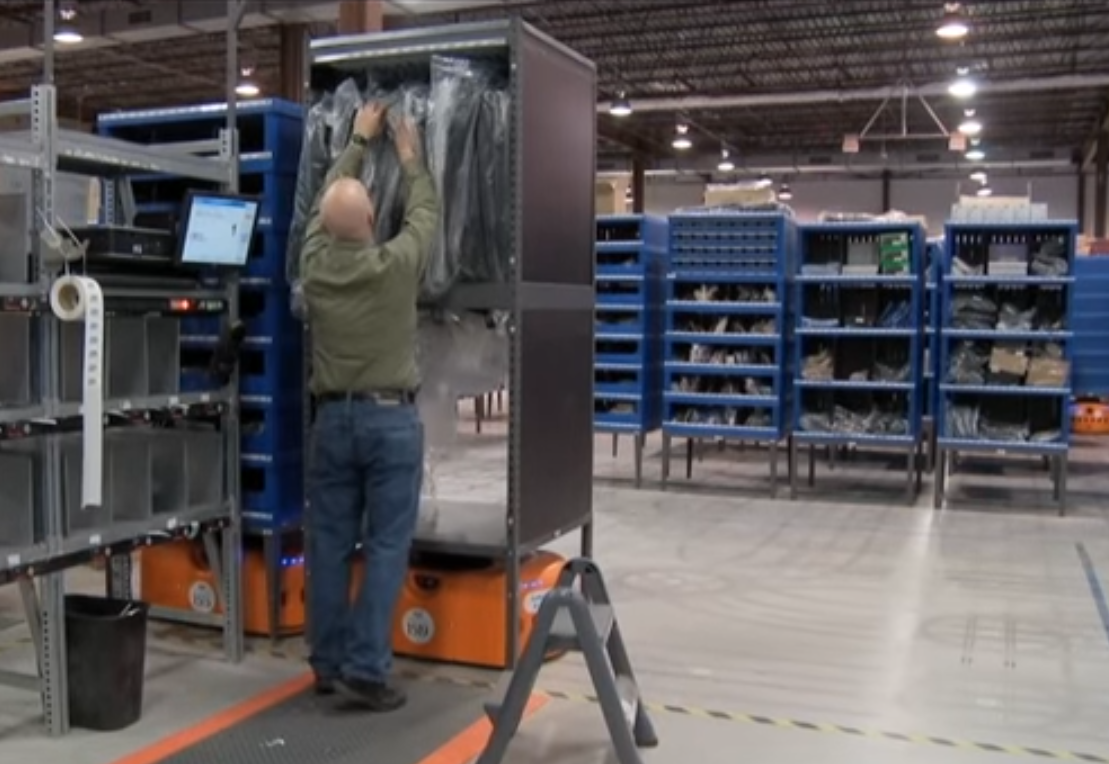
\includegraphics[width=0.8\textwidth ]{kivaprocess}
	\caption{A worker picking an order from a storage pod. Underneath, in orange is the drive unit carrying the storage pod. (\cite{kivayoutube2010quietlogistics})}
	\label{kivaprocess}
\end{figure}

\noindent The process for a drive unit is as follows:

\begin{compactenum}
	\item Unit is assigned an order
	\item Unit moves to the storage pod containing the order and picks it up
	\item Unit carries the pod to a picking station
	\item Human worker picks the order from the pod and packs the inventory
	\item Unit returns the pod back to where it was picked up
	\item Unit is assigned a new inventory
\end{compactenum}

\noindent Kiva systems do not require a complex infrastructure to operate hence solving the main issue of maintenance and operational costs. When a unit malfunctions it can be easily accessed and replaced. While malfunction occurs other units can move around it and the system remains operational. They are also very flexible and can be easily scaled as a warehouse needs only storage pods, a picking station and a number of drive units. 


\subsection{Need for the study}
%The writing includes a set of clearly articulated research questions/aims, and they are presented coherently (and hierarchically if applicable) to illustrate the structure within the questions/aims.

%Cooperative Multi-agent pathfinding has historically seen a lot of research in games but recently has risen in real world usage with robotics. Some of these fields includes disaster rescue, self-driving cars and automated ports

\textbf{HALF-DONE} Finding an optimal solution to multi-agent pathfinding is an NP-hard problem and has been research a low number of agents. Without optimization this is not an option as Warehouse Automation deals with hundreds of agents, the Office Supply company Staples uses at 500 robots in their 30000$m^{2}$ center (\cite{guizzo2008three}).

Existing literature has mainly focused on improving multi-agent pathfinding, in this project we will .

%\cite{wurman2008coordinating}



%\cite{silver2005cooperative}


%\cite{konolige2006centibots, fox2006distributed}.



\subsection{Research Aims}
\textbf{TODO} In this project we aim to reduce the complexity of Cooperative MAPF by adjusting aspects specific the to Warehouse Automation. On top of that we hope to provide a path oracle which 

\subsection{Review of the literature}
% The review’s structure clearly articulates the different levels of significance (such as general, disciplinary and/or more technical significance of the project/the field of study to which the project belongs). The review also forms a consistent and strong narrative that logically leads to the problem/gap in research that necessitates the proposed project.
% The sources used demonstrate judicious selection of literature; review exhibits perceptive interpretation of sources and clear justification for inclusion in the review.

\textbf{HALF-DONE} There are a number of problems in Warehouse Automation, some of these we will be looking at in this project include: multi-agent pathfinding, order sequencing and warehouse design.

In multi-agent pathfinding, \cite{cohen2016bounded} uses highways.

\cite{gu2010research} provides a comprehensive review of warehouse design and performance. It covers 5 major aspects, overall structure, sizing and dimensioning, department layout, equipment selection and operation strategy selection.

\cite{de2007design} provides a survey on order picking

\cite{wurman2008coordinating} provides an in depth overview of Kiva Systems, describing their benefits, usages and research areas.




\cite{ma2016optimal} presents a Conflict-Based Min-Cost-Flow algorithm which is correct, complete and optimal. It implements it on Kiva Systems looking at hundreds of agents split into dozens of teams.





%Unlike existing literature, in this project we aim looking at a number of other factors which are likely to simplify the pathfinding problem.

%Windowed Hierarchical Cooperative A∗. Cooperative A*. Conflict-Oriented Windowed Hierarchical Cooperative A∗. Compressed Path Databases.

\cite{de2007design} overview of picking

\cite{boysen2017parts} looks at the batching and sequencing of inventory orders which are given to units. Their study found that only half the units is needed when orders are optimized optimized picking allows




\section{Research Context/Background}
%This section sets the project in the context of previous studies including the most recent work.

% "Spatially Distributed Multiagent Path Planning" - region controllers - https://www.youtube.com/watch?v=-8ZsuXEwCvc&t=27s

% Cooperative problem - we are aiming to resolve conflicts to benefit the system.

% This problem is significantly harder, because the agents need to plan around both static and dynamic obstacles.

\subsection{What is Cooperative Multi-Agent pathfinding}
\noindent \textit{\textbf{I think I am missing a lot here. Not exactly sure what other background to give besides expanding on Coop MAPF}}

\textbf{TODO} Cooperative multi-agent pathfinding (MAPF) involves a number of agents in an environment moving to individual locations while avoiding collisions with one another.

Talk about: 
\begin{compactitem}
	\item NP-hard
	\item Optimality has only been done with small number of agents. Not possible here.
	\item Completeness
\end{compactitem}



\section{Research Design}
% Research design, methodology and method(s) are described with appropriate level of detail, and are presented coherently, sequentially, and/or hierarchically to illustrate the structurewithin the design. 
% Research design, methodology and method(s) are logically and consistently aligned against the relevant research questions/aims, and they are justified in light of this alignment.
% There are clear and structured descriptions, discussion and justification of timeline and administrative requirements where applicable. 

\label{Research}
\subsection{Path oracle}

\cite{strasser2015compressing}


\noindent \textbf{PLACEHOLDER} Decentralised MAPF algorithms usually involve search. A typical problem solving process (e.g. FAR (Wang \& Botea, ICAPS 2008)) involves each agent finding a path independent from all the rest (i.e. if there are k agents we solve k single-agent problems separately). When all agents have a path they each take turns moving one step at a time towards their goal. Conflicts are resolved locally choosing in favour of one agent over another in some way (e.g. assign a priority to each agent and always favour the agent with highest priority). We aim to improve efficiency by introducing a path oracle which removes entirely the need to search. The oracle is pre-computed up front and reused for every subsequent pathfinding query thereafter. Since the cost of the initial path searches tends to dominate runtime in MAPF we expect this approach will significantly improve performance. \textbf{PLACEHOLDER}

\subsection{Warehouse layout}
In many studies, the picking station is positioned on one side of the warehouse and the pods are laid out in rows (Fig. \ref{kivalayout1}).

\begin{figure}[h]
	\centering
	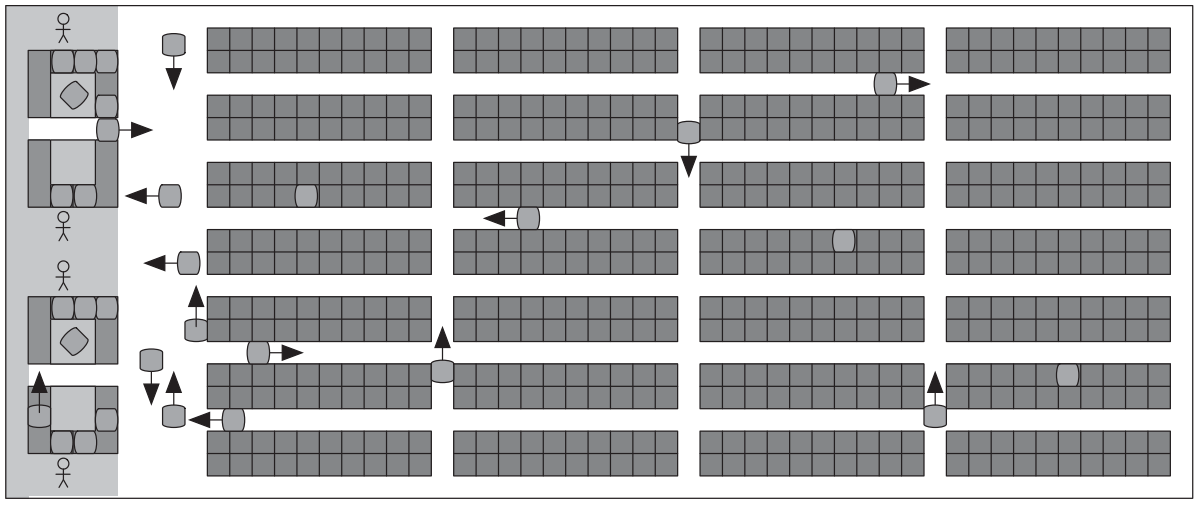
\includegraphics[width=0.9\textwidth]{kivasystemlayout}
	\caption{A Small Region of a Kiva Layout (\cite{wurman2008coordinating}). Picking stations located on the left and storage pods laid out in rows.}
	\label{kivalayout1}
\end{figure}

\cite{wilt2014spatially} looked at identifying zones by areas which are bottlenecks and assigning a controller, for that zone which manages any agents who need to travel through the bottleneck. Inspired by this and assuming pickup stations, we plan to split the warehouse into two halves and introduce an intermediate zone (See Fig \ref{kivalayout2}). Delivering pods which are situated in the far zone is a two step process:
\begin{compactenum}
	\item Units in the far zone move pods to the intermediate zone instead of a pickup station
	\item Units in the delivery zone will pickup pods in the intermediate zone
\end{compactenum}
\noindent These zones will have their own controller which handles any agents within the zone and tells them what behaviour should occur.

\begin{figure}[h]
	\centering
	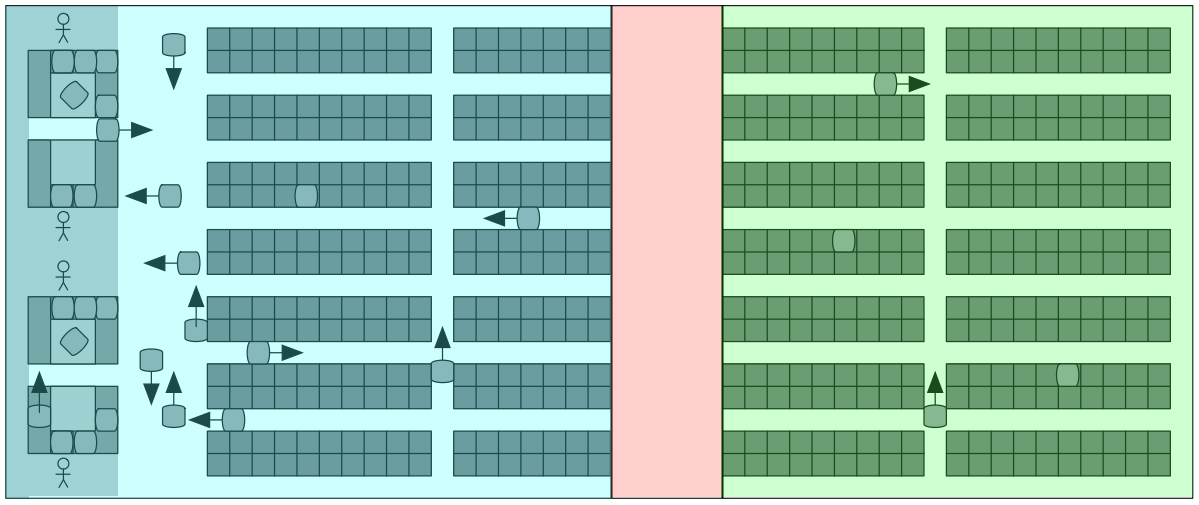
\includegraphics[width=0.9\textwidth]{kivasystemlayout_adjusted}
	\caption{Intermediate zone in red, delivery zone in blue and far zone in green}
	\label{kivalayout2}
\end{figure}

\subsection{Order picking}
As pods can be dynamically move around the warehouse, the layout pods can be changed to suit incoming orders. Storage pods containing popular orders may be placed next to a picking station so a drive unit can readily access it and unpopular orders will be placed further away. Vice-versa the distribution of orders can be re-ordered to suit the current layout of the warehouse. Here we may take inspiration from Robin-hood hashing and apply it to sorting the inventory pods. \cite{boysen2017parts} covered both of these aspects in detail and revealed that after optimizing orders, the total number of drive units can be cut by half and retain the same supply to picking stations.

% proving that the problem is NP-hard for even a single order and that their solution is strongly NP-complete.

\subsection{Allowing for movement underneath storage pods}
As drive units are capable of moving underneath pods when carrying them, this means that with small adjustments to the dimensions of storage pods it is possible to allow drive units to maneuver underneath the pods. With this the only obstacles in the environment are other drive units.

\subsection{Timetable/plan}
\textbf{HALF DONE}
\begin{center}
{\footnotesize
\begin{tabular}{ c p{12cm} }
\multicolumn{2}{l}{\textbf{Semester 1}} \\
\hline \multicolumn{1}{c}{Week(s)} & \multicolumn{1}{c}{Plan} \\
\hline 7  & Model warehouse and simple A* pathfinding \\
\hline 8  & Add multiple agents with A* assigned random pods (no picking station) arsasarsa\\
\hline 9  & Implement Cooperative A* \\
\hline 11 & Add simple scheduler which assigns agents a location to fetch a random pod and return to the picking station \\
\hline 12 & Focus on Interim Presentation \\
\hline 13 & Focus on Literature Review \\
\hline 14 & Focus on Examinations \\
\hline Holidays & Implement Path Oracle with Compressed Path Databases \\
\hline
\end{tabular}
}


{\footnotesize
\vspace{0.5cm}
\begin{tabular}{ c p{12cm} }
\multicolumn{2}{l}{\textbf{Semester 2}} \\
\hline \multicolumn{1}{c}{Week(s)} & \multicolumn{1}{c}{Plan} \\
\hline 1  & Add more complex scheduler, distributing requested inventory  and allow agents dynamically sort pods according to popularity. Agents dynamically sort pods according to popularity. Decide on the focus for the rest of the project. \\
\hline 2-4 & Implement Path Oracle with Compressed Path Databases \\
\hline 3  &  \\
\hline 4  & \\
\hline 5  &   \\
\hline 6  &  \\
\hline 7  & \\
\hline 8  & \\
\hline 9  & \\
\hline 10 & \\
\hline 11 & \\
\hline 12 & Finish Final Thesis \\
\hline 13 & Additional tasks \\
\hline 14 & Focus on Final Presentation \\
\hline 15 & Focus on Final Thesis \\
\hline
\end{tabular}
}
\end{center}


\section{Significance / Expected Outcomes of the study}
% (Expected) outcomes of the project are discussed with appropriate level of detail, and are presented coherently to illustrate varying levels of implications and contributions the project offers. 
% (Expected) outcomes are logically and consistently aligned against the relevant research questions/aims

\textbf{TODO}


\noindent \textbf{Contributions}
\begin{compactitem}
	\item A Warehouse Automation simulation
	\item A better understanding of the effects of Warehouse Configurations
	\item An improved MAPF solution utilizing a path oracle
\end{compactitem}


We should have a better understanding of how the aspects described in Section \ref{Research} affect the performance of Warehouse Automation.

Increased inventory supply for the picking stations. Decreasing speed for MAPF calculations.

%\section{Glossary of terms} % Temporary, delete later

%\begin{enumerate}
%	\item avoidance
%	\item path planning
%	\item Drive Unit Agent (DUA)
%	\item Storage Pod
%	\item Makespan
%	\item Idle time
%	\item Performance curve relative to..?
%	\item Robin-hood hashing
%   \item order distribution systems
%\end{enumerate}

\bibliographystyle{dcu}
\bibliography{bibliography}


\end{document}
